\documentclass{article}

\setlength{\headsep}{0.75 in}
\setlength{\parindent}{0 in}
\setlength{\parskip}{0.1 in}

%=====================================================
% Add PACKAGES Here (You typically would not need to):
%=====================================================

\usepackage{xcolor}
\usepackage[margin=1in]{geometry} % Used for page margins, often replaces fullpage
\usepackage{amsmath,amsthm,amssymb} % amssymb added for common math symbols

\usepackage{enumitem} % For custom list environments

\usepackage{tcolorbox}
% \usepackage{fullpage} % Geometry handles this better
\usepackage[parfill]{parskip} % For paragraph spacing
\usepackage{hyperref}
\usepackage[nameinlink, capitalise]{cleveref} % For smart referencing

\usepackage{algorithm2e} % For algorithms
\usepackage{tikz} % For drawing diagrams
\usepackage{siunitx} % For units
\usepackage{graphicx}
\usepackage{float}

\usetikzlibrary{arrows.meta, positioning}

\crefname{algocf}{Algorithm}{Algorithms}

\RestyleAlgo{ruled} % Style for algorithms

\definecolor{linkc}{rgb}{0.1, 0.5, 0.7}
\definecolor{citec}{rgb}{0.6, 0.3, 0.7}
\definecolor{urlc}{rgb}{0.5, 0.1, 0.2}
\hypersetup{
  colorlinks=true,
  linkcolor=linkc,
  citecolor=citec,
  urlcolor=urlc
}

\renewcommand{\d}{\,\mathrm{d}} % Differential d

%=====================================================
% Ignore This Part (But Do NOT Delete It:)
%=====================================================

\theoremstyle{definition}
\newtheorem{problem}{Problem}
\newtheorem*{fun}{Fun with Algorithms}
\newtheorem*{challenge}{Challenge Yourself}
\def\fline{\rule{0.75\linewidth}{0.5pt}}
\newcommand{\finishline}{
  \begin{center}\fline
\end{center}}
\newtheorem*{solution*}{Solution}
\newenvironment{solution}{
\begin{solution*}}{{\finishline}
\end{solution*}}
\newcommand{\grade}[1]{\hfill{\textbf{($\mathbf{#1}$ points)}}}
\newcommand{\thisdate}{\today}
\newcommand{\thissemester}{\textbf{Rutgers: Spring 2026}}
\newcommand{\thiscourse}{CS 344: Algorithms}
\newcommand{\thishomework}{Number}
\newcommand{\thisname}{Name}
\newcommand{\thisextension}{Yes/No}

\headheight 40pt
\headsep 10pt

\newcommand{\headrulewidth}{0pt}

\newcommand{\thisheading}{
  \noindent
  \begin{center}
    \framebox{
      \vbox{\vspace{2mm}
        \hbox to 6.28in { \textbf{\thiscourse \hfill \thissemester} }
        \vspace{4mm}
        \hbox to 6.28in { {\Large \hfill Homework \#\thishomework \hfill} }
        \vspace{2mm}
        \hbox to 6.28in { { \hfill \hfill} }
        \vspace{2mm}
        \hbox to 6.28in { \emph{Name(s): \thisname \hfill }}
      \vspace{2mm}}
    }
  \end{center}
  \bigskip
}

%=====================================================
% Some useful MACROS (you can define your own in the same exact way also)
%=====================================================

\newcommand{\ceil}[1]{{\left\lceil{#1}\right\rceil}}
\newcommand{\floor}[1]{{\left\lfloor{#1}\right\rfloor}}
\newcommand{\prob}[1]{\Pr\paren{#1}}
\newcommand{\expect}[1]{\Exp\bracket{#1}}
\newcommand{\var}[1]{\textnormal{Var}\bracket{#1}}
\newcommand{\set}[1]{\ensuremath{\left\{ #1 \right\}}}
\newcommand{\poly}{\mbox{\rm poly}}

%=====================================================
% Fill Out This Part With Your Own Information:
%=====================================================

\renewcommand{\thishomework}{1} %Homework number
\renewcommand{\thisname}{Iris$_1$ Martinez$_1$} % Enter your name here

\begin{document}

\thisheading

\subsection*{Homework Policy}
\begin{itemize}
  \item You may consult all course materials (lecture notes, textbook, slides, etc.) while writing your solutions. No external resources are permitted.

  \item \textbf{All submissions should be typeset in LaTeX, handwritten solutions are not accepted}.

  \item Remember to always \textbf{prove the correctness} of your algorithms and \textbf{analyze their running time} (or any other efficiency measure asked in the question).

  \item Homework assignments are completed and submitted in fixed groups of 3 students. Only \textbf{one member of the group submits} the full solution on Canvas. The submission must include the names of all group members. The other two members do \textbf{not need to submit anything separately}.

  \item You may discuss the problems with any of your classmates, even those outside your group. However, \textbf{each group must write and submit their solutions independently}.

  \item  Attempt the challenge problems only if you find them interesting.
\end{itemize}

\subsection*{Acknowledgment (to be reviewed and edited as needed)}
\begin{tcolorbox}[colframe=black,colback=white,arc=5mm]
  I, \textbf{Iris Martinez (bam322)}, completed this assignment individually. For assitance in LaTeX typesetting, I referred to Gemini 3 Pro for assitance.For problem 1, I made use of a graphing calculator to inform my observations of function behavior and guide my proofs. In part c of problem 1, I referenced the wikipedia page on the stirling approximation of factorials. In problem 2, i made use of the algorithms book when i forgot the details of solving recursion trees.\textbf{I hereby affirm that all external assistance utilized in the preparation of this document has been properly acknowledged}.
\end{tcolorbox}

\finishline
\newpage

\newpage

\bigskip

\begin{problem}
  This question reviews asymptotic notation. You may assume the following inequalities for this question (and throughout the course): For any \underline{constant} $c \geq 1$,
  \begin{align*}
    (\log{n})^c = o(n) \quad,\quad n^c = o(n^{c+1}) \quad,\quad c^n = o((c+1)^n) \quad,\quad (n/2)^{(n/2)} = o(n!).
  \end{align*}
  \begin{enumerate}
    \item[(a)] Rank the following functions based on their asymptotic value in increasing order, i.e., list them as functions $f_1,f_2,f_3,\ldots,f_{14}$ such that $f_1 = O(f_2)$, $f_2 = O(f_3), \ldots, f_{13} = O(f_{14})$. Remember to write down your proof
      for each equation $f_i = O(f_{i+1})$ in the sequence above.  \grade{20}
      \begin{align*}
        &\log^3 n &&\frac{n}{\log n} &&\sqrt{n}  &&n^2  &&n^{\log n} \\
        &n^{1.5} &&e^{\sqrt{n}} &&e^n &&n!  &&2^{n^2} \\
        &3^n && 10^{n} &&n^n &&(\log n)^{\log n} &&n^{\log \log n}
      \end{align*}

      \smallskip
      \emph{Hint:} For some of the proofs, you can simply show that $f_i(n) \leq f_{i+1}(n)$ for all \underline{sufficiently large} $n$ which immediately implies $f_i = O(f_{i+1})$.

      %=====================================================
      % LaTeX Tip: Write your solutions for each problem in a solution environment, i.e., between a \begin{solution} and \end{solution} command. For problems that have multiple part, use this command right after each part
      % of the problem.
      %=====================================================

      \begin{solution}
        \
        \begin{itemize}
          \item \textbf{Smallest}
          \item $\log^3 n$ because $log^3 n$ is $O(\sqrt{n}).$

            My proof is as follows:
            \

            $\sqrt{n} - \log^3(n) >= 0$ This statement claims that $\sqrt(n)$ is bigger than $\log^3(n)$. We will solve to find if there exists a solution to this inequality.

            $n - (\log^3(n))^2 >=0$

            $n - (\log^6(n)) >= 0$

            $n >= \log^6 n$

            $ n^{1/6} >= \log n$

            $ b^{n^{1/6}} >= n$

            We know have an equaiton we can solve for all positive n for a base b that makes $ b^{n^{1/6}}$ greater than or equal to n and therefore we have proven that $\sqrt{n}$ will always domiante $\log^3 n$ as n goes to infinity.
          \item $\sqrt{n}$

            My proof is as follows:

            $\sqrt{n} = O(\frac{n}{\log{n}})$ because $\log{n}$ becomes irrelevant to n as n goes to infinity. So $\frac{n}/log{n}$ looks linear. Linear functions are always larger than square root ones, so $\sqrt{n} = O(\frac{n}{\log n})$
          \item $\frac{n}{\log n}$

            My proof is as follows:

            $\frac{n}{\log n} = O(n^{1.5})$ because $\frac{n}{\log n}$ performs linearly in the limit, where $n^{1.5}$ is exponential.
          \item $n^{1.5}$

            My proof is as follows:

            $n^{1.5} = O(n^2)$ because they have the same base but the exponent $2>1.5$
          \item $n^2$

            My proof is as follows:

            $n^2 = O(\log n^{\log n})$ because as n goes to infinity, we are comparing $n*n$ with $ ({\log n})_1 * ({\log n})_2 * ... * ({\log n})_{\log n}$

            If we use the heuristic understanding that more multiplications makes for a larger function, can see how in the limit we are multiplying $\log n$ so many more times that the large value for n is irrelevant.

            We can also look at this algebraically like this:

            $ n^2 = (\log n)^{\log n}$

            $ln (n^2) = ln((\ln n) ^ {ln n})$
            $2*ln(n) = \ln n * (\ln \ln n)$

            $ 2= \ln \ln n$

            2 is less than $\ln \ln n$ in the limit so we prove $(\log n)^{log n}$ is bigger
          \item $(\log n)^{\log n}$

            $(\log n)^{\log n}$ is $\theta(n^{\log \log n})$

            My proof is as follows:

            $(\log n) ^ {\log n} = n^{\log \log n}$

            $(\log n) = n^{\frac{\log \log n}{\log n}}$

            $(\log n) = n^{\log_n \log n}$

            $\log n = \log n$

            This shows that the functions are equal and therefore they have a $\theta$ relationship
          \item $n^{\log \log n}$

            My proof is as follows:

            $n^{\log \log n} = O(n^{\log n})$ because they have the same base but $\log n$ will always be a bigger exponent than $\log \log n$
          \item $n^{\log n}$

            My proof is as follows:

            $ e ^{\sqrt {n}} = n^{\ln n}$

            $ \ln (e ^{\sqrt {n}}) = \ln(n^{\ln n})$

            $ \sqrt {n} = \ln^2 n$

            $ n^{\frac{1}{4}} = \ln n$

            $ \lim_{x \to \infty} \frac{n^{\frac{1}{4}}}{\ln n} = \infty$ We now apply l'hopital's

            $ \lim_{x \to \infty} \frac{\frac{1}{4}n^{-{3/4}}}{\frac{1}{n}}$ I skip some steps for brevity

            $ \lim_{x \to \infty} \frac{n^{\frac{1}{4}}}{4} = \infty$ Which shows that the $e^{\sqrt{n}}$ is bigger
          \item $e^{\sqrt{n}}$

            My proof is as follows:

            $e^{\sqrt{n}} = O(e^n)$ because $n>\sqrt{n}$
          \item $e^n$

            My proof is as follows:

            $ e^n = O(3^n)$ because $3>e$
          \item $3^n$

            My proof is as follows:

            $ e^n = O(10^n)$ because $10>3$
          \item $10^{n}$

            My proof is as follows:
            $10^n = O(n!)$ because as n goes to infinity we begin to multiply by numbers much larger than 10 a very large number of times, causing us to overtake the constant multiplication by a factor of 10 of $10^n$

          \item $n!$

            My proof is as follows:

            n factorial multiplies n times by numbers that steadily get smaller than n. $n^n$ multiplies by exactly n just as many times as n factorial. Therefore it must always be bigger.

          \item $n^n$

            My proof is as follows:

            $log n^n = log (2^{n^2})$ if we ignore the bases we get

            $ n = 2^n$

            Which is clearly bigger than just n
          \item $2^{n^2}$
          \item \textbf{Largest}
        \end{itemize}
      \end{solution}

    \item[(b)]  Consider the following four different functions $f(n)$:
      \begin{align*}
        1 \qquad\qquad  \log^4{n} \qquad\qquad  n^{\sqrt{\log n}}  \qquad\qquad 5^{n^3}.
      \end{align*}
      For each of these functions, determine which of the following statements is true and which one is false. Remember to write down your proof for each choice.    \grade{10}
      \begin{itemize}
        \item $f(n) = \Theta(f(n-1))$;
        \item $f(n) = \Theta(f(\frac{n}{2}))$;
        \item $f(n) = \Theta(f(\sqrt n))$;
      \end{itemize}

      \smallskip
      \textbf{Example:} For the function $f(n) = 5^{n^3}$, we have $f(n-1) = 5^{(n-1)^3}$. Expanding,
      \[
        5^{(n-1)^3} = 5^{n^3 - 3n^2 + 3n - 1} = \frac{5^{n^3}}{5^{3n^2 - 3n + 1}}.
      \]
      Thus,
      \[
        \lim_{n \to \infty}\frac{f(n)}{f(n-1)} = \lim_{n \to \infty} \frac{5^{n^3}}{5^{n^3 - 3n^2 + 3n - 1}} = 5^{3n^2 - 3n + 1} \to \infty.
      \]
      As such, $f(n) \neq O(f(n-1))$ and the first statement is false for $5^{n^3}$.

      \begin{solution}
        \

        \begin{itemize}
          \item $f(n) = 1$
            \begin{itemize}
              \item For all of of the listed statements, they are true. As a constant function, $f(n) = 1$ is going to be $\theta(f(x))$ where $f(x)$ can be anything.
            \end{itemize}
          \item $f(n) = (\log n)^4$
            \begin{itemize}

              \item $f(n) = \theta(f(n-1))$

                $\lim_{n \to \infty}\frac{(\log n)^4}{(\log (n-1))^4} \approx 1$

                Therefore, $f(n) = \theta(f(n-1))$
              \item $f(n) = \theta(f(n/2))$

                $\lim_{n \to \infty}\frac{(\log n)^4}{(\log (n/2))^4}$

                $\lim_{n \to \infty}\frac{(\log n)}{(\log n) - \log 2} \approx 1$

                Therefore, $f(n) = \theta(f(n/2))$
              \item $f(n) = \theta(f(\sqrt{n}))$

                $\lim_{n \to \infty}\frac{(\log n)^4}{(\log (\sqrt{n}))^4}$

                $\lim_{n \to \infty}\frac{\log n}{\log n^{\frac{1}{2}}} \approx 2$

                Therefore, $f(n) = \theta(f(\sqrt{n}))$
            \end{itemize}
          \item $f(n) = n^{\sqrt{\log n}}$
            \begin{itemize}
              \item $f(n) = \theta(f(n-1))$

                $\lim_{n \to \infty}\frac{n^{\sqrt{\log n}}}{n^{\sqrt{\log n-1}}} \approx 0$

                Therefore, $f(n) = \theta(f(n-1))$
              \item $f(n) \neq \theta(f(\frac{n}{2})$

                  $\lim_{n \to \infty}\frac{n^{\sqrt{\log n}}}{n^{\sqrt{\log \frac{n}{2}}}}$

                  $\lim_{n \to \infty}\frac{n^{\sqrt{\log n}}}{n^{\sqrt{\log \frac{n}{2}}}} = \infty$

                  Therefore, $f(n) \neq \theta(f(\frac{n}{2}))$
                \item $f(n) \neq \theta(f(\sqrt{n})$

                    $\lim_{n \to \infty}\frac{n^{\sqrt{\log n}}}{n^{\sqrt{\log \sqrt{n}}}}$

                    $\lim_{n \to \infty}\frac{n^{\sqrt{\log n}}}{n^{\sqrt{\log \sqrt{n}}}} = \infty$

                    Therefore, $f(n) \neq \theta(f(\sqrt{n}))$
                \end{itemize}
              \item $f(n) = 5^{n^{3}}$
                \begin{itemize}
                  \item $f(n) \neq \theta(f(n-1))$ Given.
                  \item $f(n) \neq \theta(f(\frac{n}{2}))$

                    $\lim_{n \to \infty}\frac{5^{n^3}}{5^{\frac{n}{2}^3}}$

                    $\lim_{n \to \infty}\frac{5^{n^3}}{5^{\frac{n^3}{8}}}$

                    $\lim_{n \to \infty}\frac{5^{n^3}}{5^{\frac{n^3}{8}}} = \infty$

                    Therefore, $f(n) \neq \theta(f(\frac{n}{2}))$

                  \item $f(n) \neq \theta(f(\sqrt{n}))$

                    $\lim_{n \to \infty}\frac{5^{n^3}}{5^{\sqrt{n}^3}}$

                    $\lim_{n \to \infty}\frac{5^{n^3}}{5^{\frac{3}{2}}}$

                    $\lim_{n \to \infty}\frac{5^{n^3}}{5^{\frac{3}{2}}} = \infty$

                    Therefore, $f(n) \neq \theta(f(\sqrt{n}))$
                \end{itemize}
            \end{itemize}
          \end{solution}

        \item[(c)] For each of the following functions, state whether $f(n) = O(g(n))$ or $f = \Omega(g(n))$, or if both are true, then write $f = \Theta(g(n))$. No proofs required for this problem.  \grade{15}
          \begin{enumerate}
            \item $f(n) = \sum_{k=1}^{n} \log k$ and $g(n) = \log(n!)$
            \item $f(n) = n^{\log_3(n)}$ and $g(n) = n^{\sqrt{\log n}}$
            \item $f(n) = \sum_{k=1}^{n} k^2$ and $g(n) = n^3$
            \item $f(n) = 2^{\sqrt{n \log n}}$ and $g(n) = 3^{\sqrt{n}}$
            \item $f(n) = n^{\log n}$ and $g(n) = n^{\log \log n}$
            \item $f(n) = 10^n$ and $g(n) = n^{n/2}$
            \item $f(n) = n!$ and $g(n) = (n/e)^n$
            \item $f(n) = \sum_{k=1}^{n} k \log k$ and $g(n) = \frac{n^2}{\log n}$
            \item $f(n) = (\log n)^{\log n}$ and $g(n) = 2^{\log n}$
            \item $f(n) = e^{\sqrt{n}}$ and $g(n) = 2^n$
          \end{enumerate}

      \end{enumerate}
    \end{problem}

    \begin{solution}
      \begin{enumerate}
        \item $f(n) = \theta(g(n))$
        \item $f(n) = \omega(g(n))$
        \item $f(n) = \theta(g(n))$
        \item $f(n) = \omega(g(n))$
        \item $f(n) = \omega(g(n))$
        \item $f(n) = O(g(n))$
        \item $f(n) = \omega(g(n))$
        \item $f(n) = \omega(g(n))$
        \item $f(n) = \omega(g(n))$
        \item $f(n) = O(g(n))$
      \end{enumerate}
    \end{solution}

    \newpage

    \begin{problem}
      Your goal in this problem is to analyze the \emph{runtime} of the following (imaginary) recursive algorithms for some (even more imaginary) problem:
      \begin{enumerate}[label=(\Alph*)]

        \item  Algorithm $A$ divides an instance of size $n$ into $5$ subproblems of size $n/5$ each, recursively solves each one, and then takes $O(n)$ time
          to combine the solutions and output the answer.

          \begin{solution}

            %=====================================================
            % LaTeX Tip: The figure environment is used for displaying the figure. Inside that, we use \includegraphics for adding a different file for each of the figure.
            % What you need to do is to create your figure using any tool you like (including drawing it by hand and scanning it), turn it into a pdf, name it "tree[X].pdf"
            % where you replace [X] by A,B,C, or D depending on which part you are solving (i.e., use treeA.pdf, treeB.pdf,...). Finally, copy the file in the same directory
            % as this template and you should see that getting compiled into your solution. You can change the width=0.5\textwidth command to fix the size of the figure
            % in the final PDF. Finally, if the figure appears in the next page, do not worry about it as they will still have the proper caption.
            %=====================================================
            \begin{figure}[H]
              \centering
              \IfFileExists{problemA.pdf}{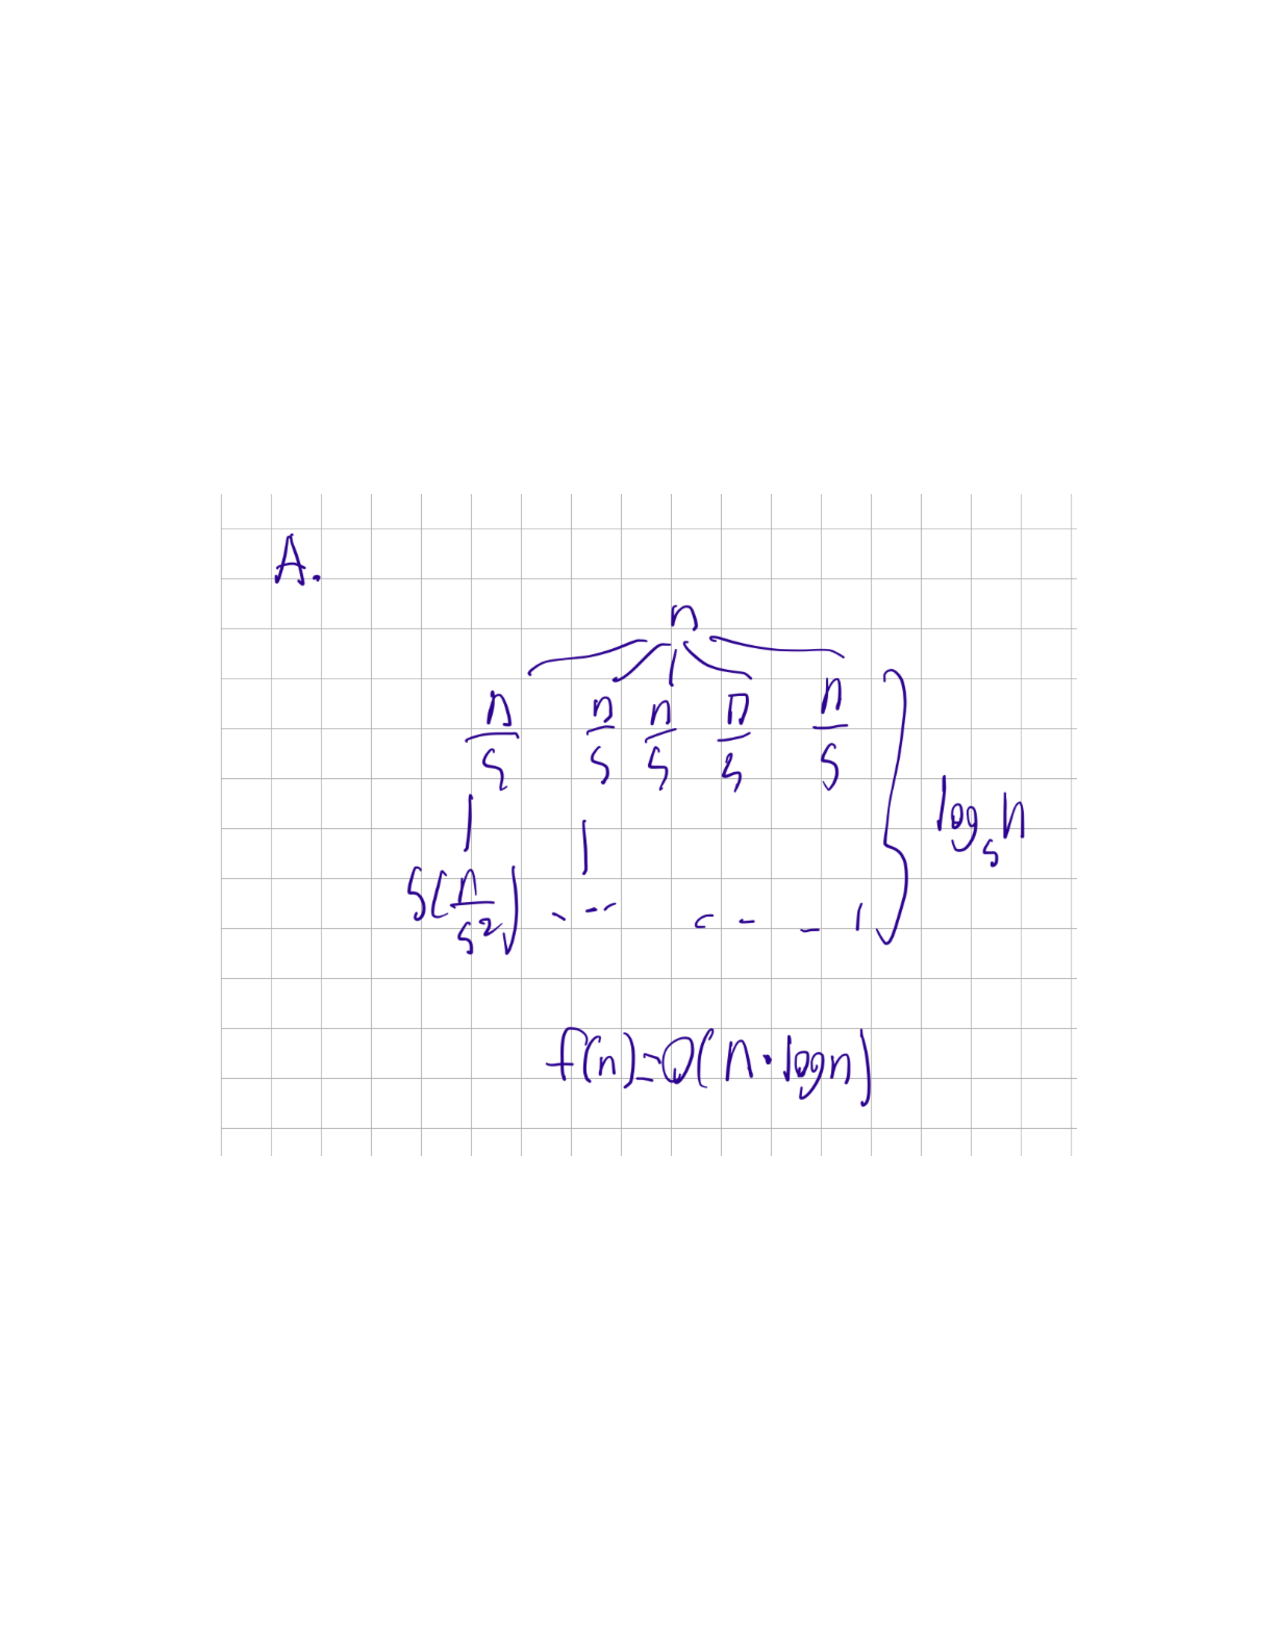
\includegraphics[width=0.5\textwidth]{problemA.pdf}}{No Figure Yet}
              \caption{Recursion tree for algorithm $A$.}
            \end{figure}

          \end{solution}

        \item Algorithm  Algorithm $B$ divides an instance of size $n$ into $5$ subproblems of size $n/2$ each, recursively solves each one, and then takes $O(n^2)$ time
          to combine the solutions and output the answer.

          \begin{solution}
            \begin{figure}[H]
              \centering
              \IfFileExists{problemB.pdf}{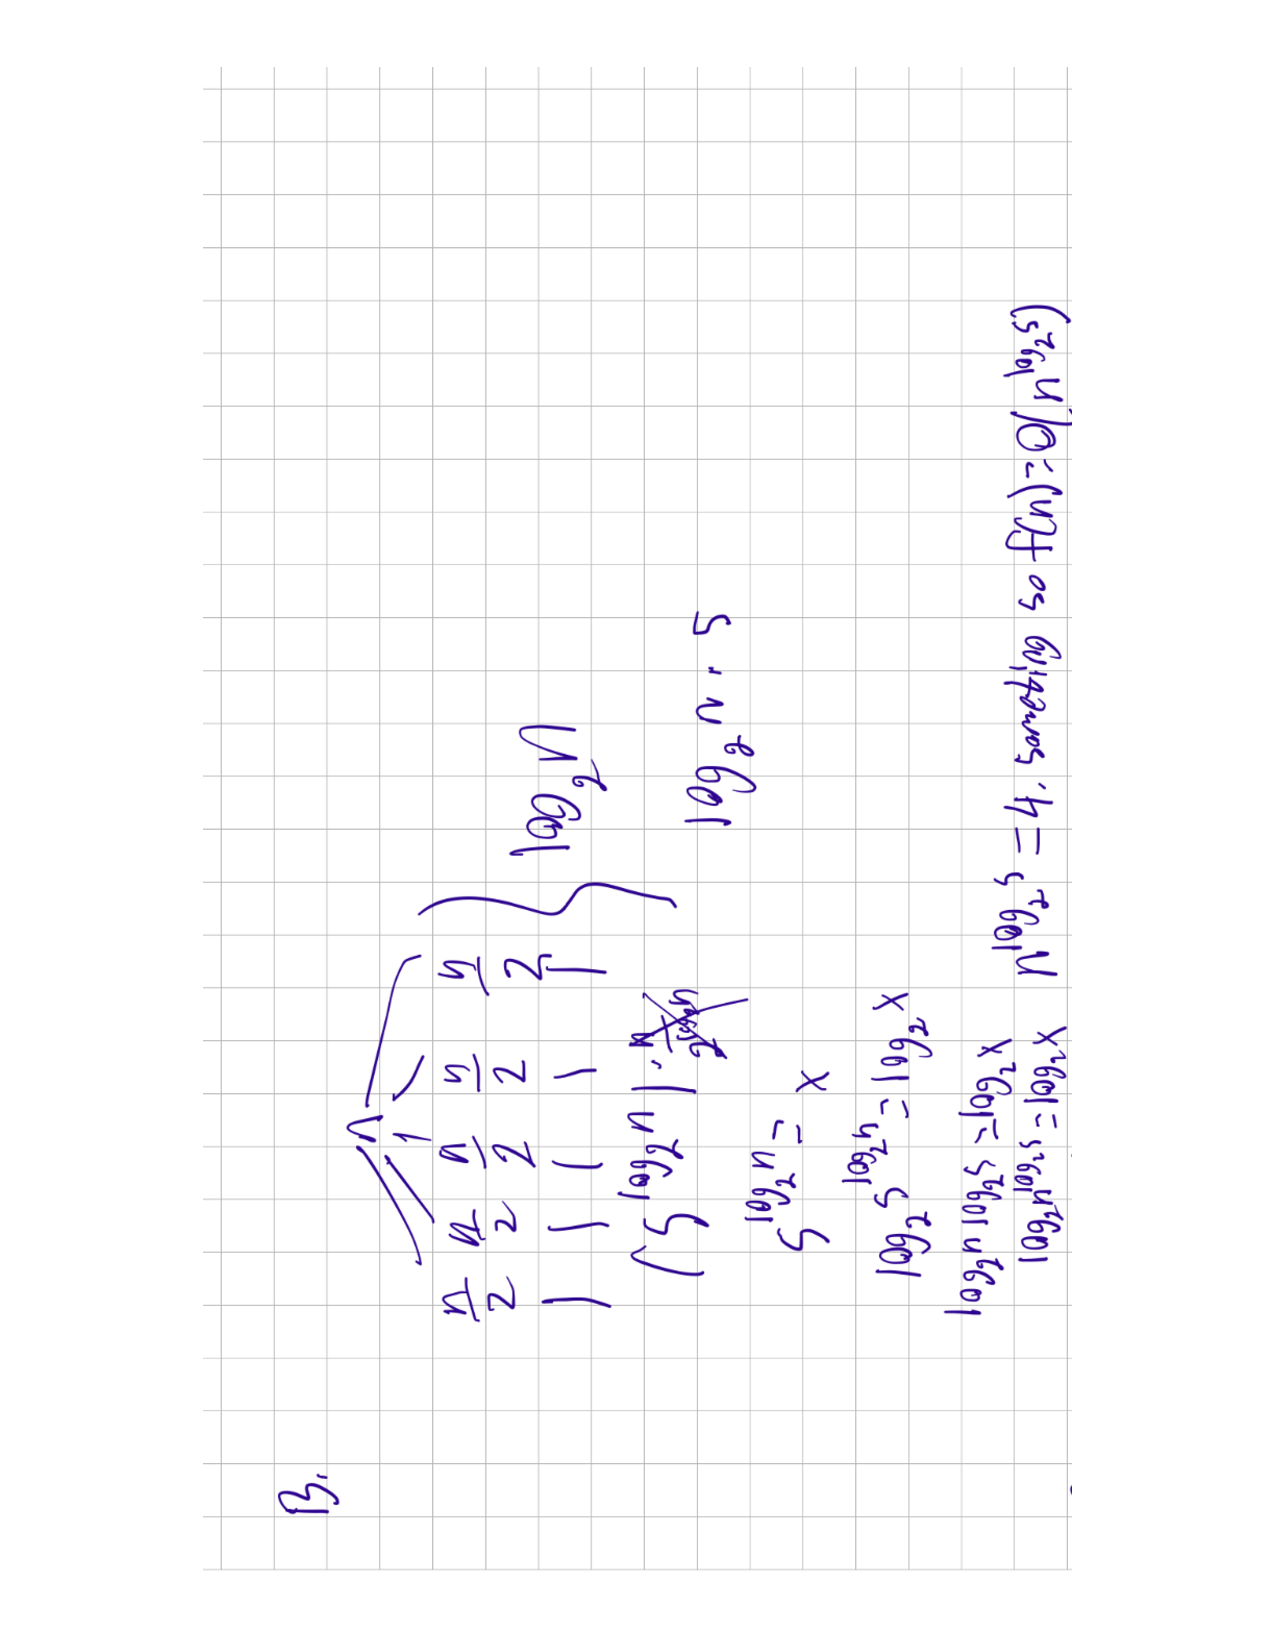
\includegraphics[width=0.5\textwidth]{problemB.pdf}}{No Figure Yet}
              \caption{Recursion tree for algorithm $B$.}
            \end{figure}
          \end{solution}

        \item Algorithm $C$ divides an instance of size $n$ into $5$ subproblems of size $n/2$ each, recursively solves each one, and then takes $O(n^{0.8})$ time
          to combine the solutions and output the answer.
          \begin{solution}
            Solution to part (c) goes here. % Delete this line and write your own solution here.

            \begin{figure}[H]
              \centering
              \IfFileExists{problemC.pdf}{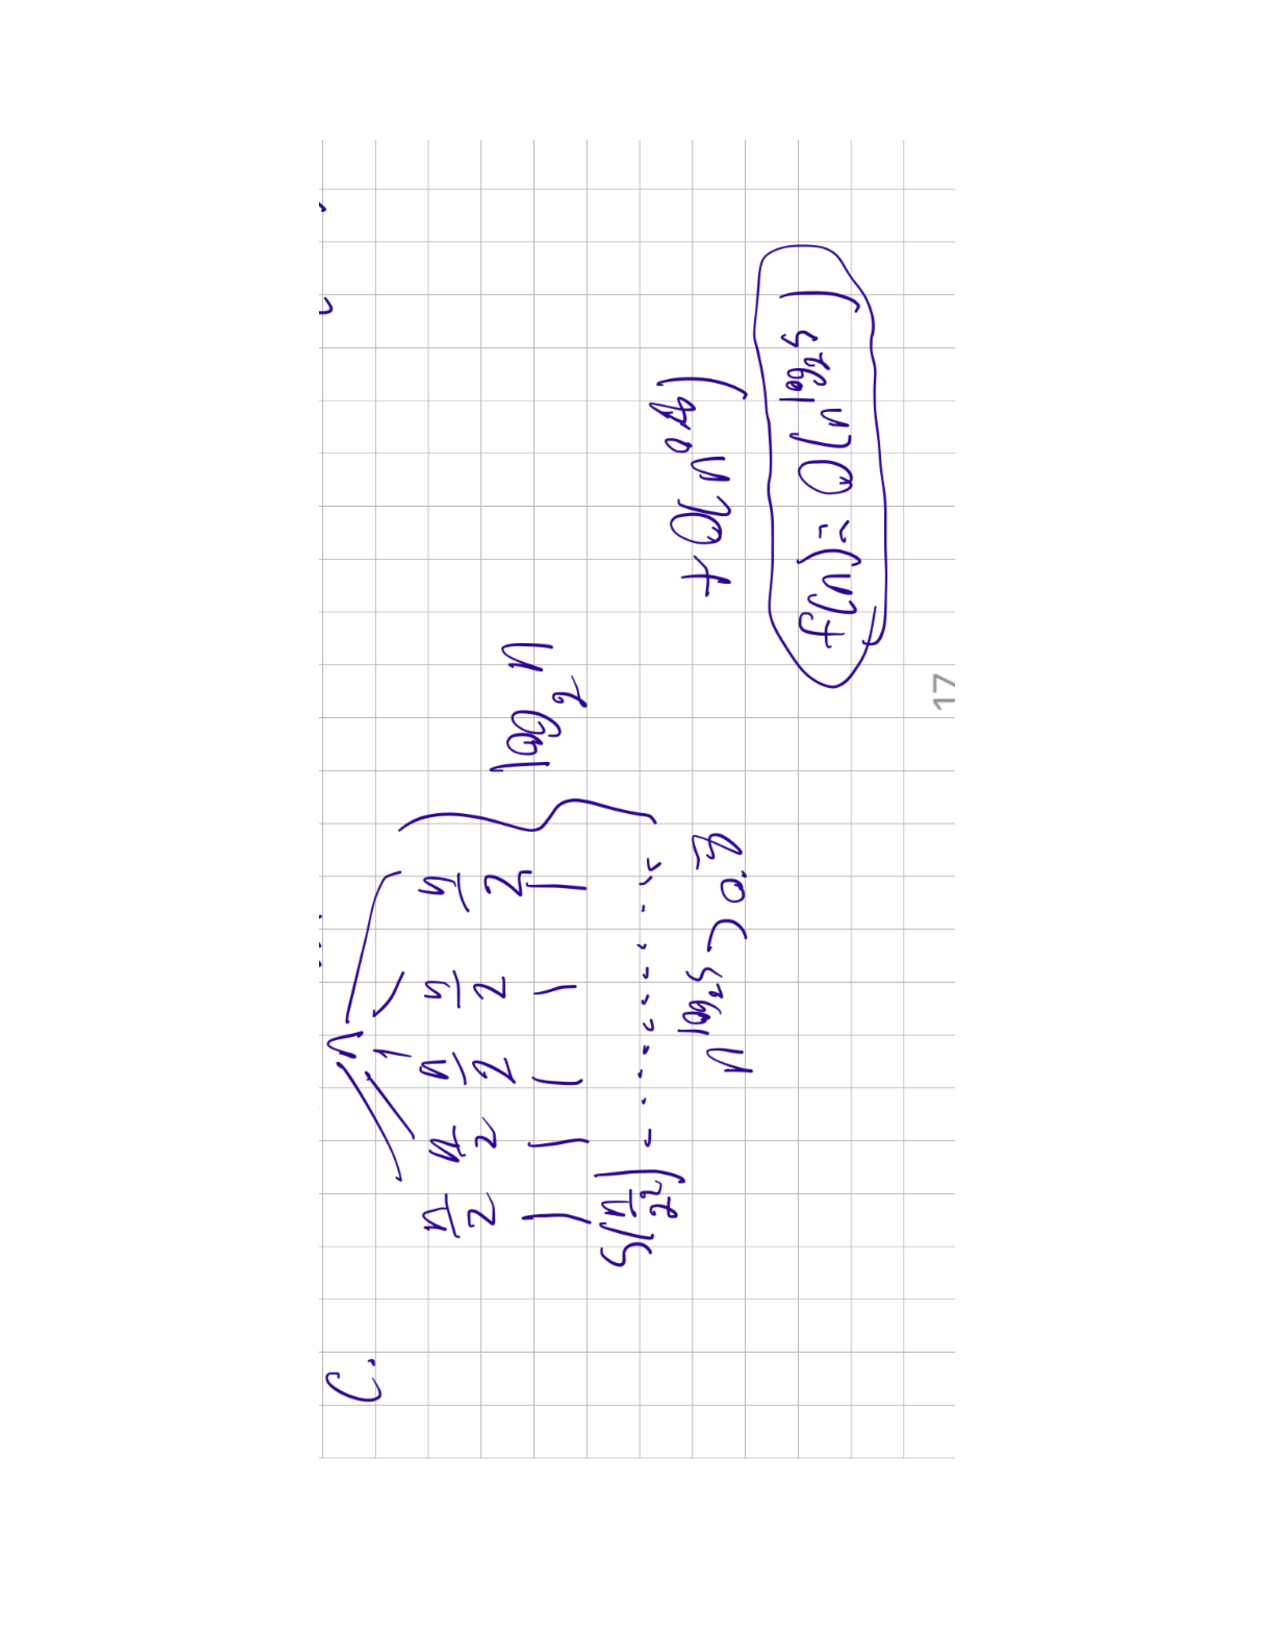
\includegraphics[width=0.5\textwidth]{problemC.pdf}}{No Figure Yet}
              \caption{Recursion tree for algorithm $C$.}
            \end{figure}
          \end{solution}

        \item $D$ divides an instance of size $n$ into $2$ subproblems, one with size $n/4$ and one with size $n/5$, recursively solves each one, and then takes $O(n)$ time
          to combine the solutions and output the answer.

          \begin{solution}
            Solution to part (d) goes here. % Delete this line and write your own solution here.

            \begin{figure}[H]
              \centering
              \IfFileExists{problemD.pdf}{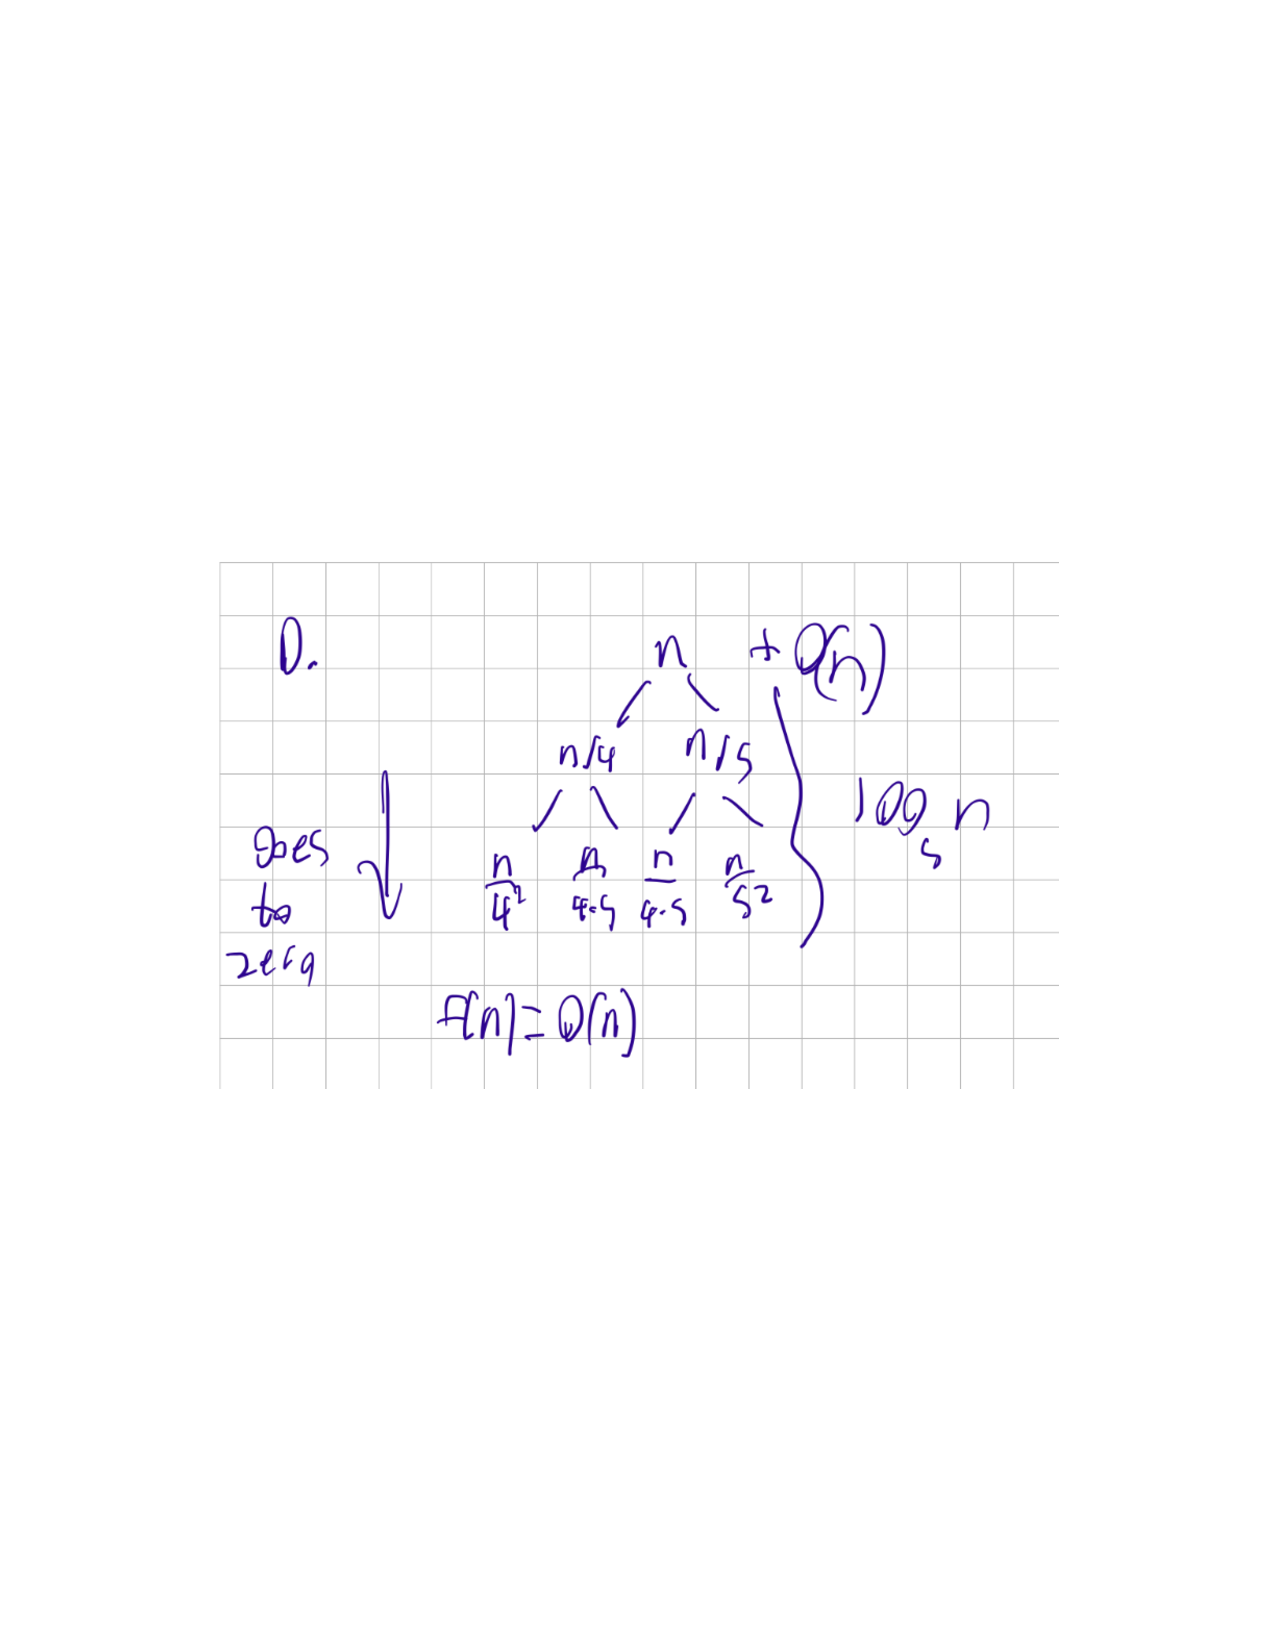
\includegraphics[width=0.5\textwidth]{problemD.pdf}}{No Figure Yet}
              \caption{Recursion tree for algorithm $D$.}
            \end{figure}

          \end{solution}

        \item Algorithm $E$ divides an instance of size $n$ in to $3$ subproblems of size $n-1$ each, recursively solves each one, and then takes $O(1)$ time to combine the solutions and output the answer.

          \begin{solution}
            Solution to part (e) goes here. % Delete this line and write your own solution here.

            \begin{figure}[H]
              \centering
              \IfFileExists{problemE.pdf}{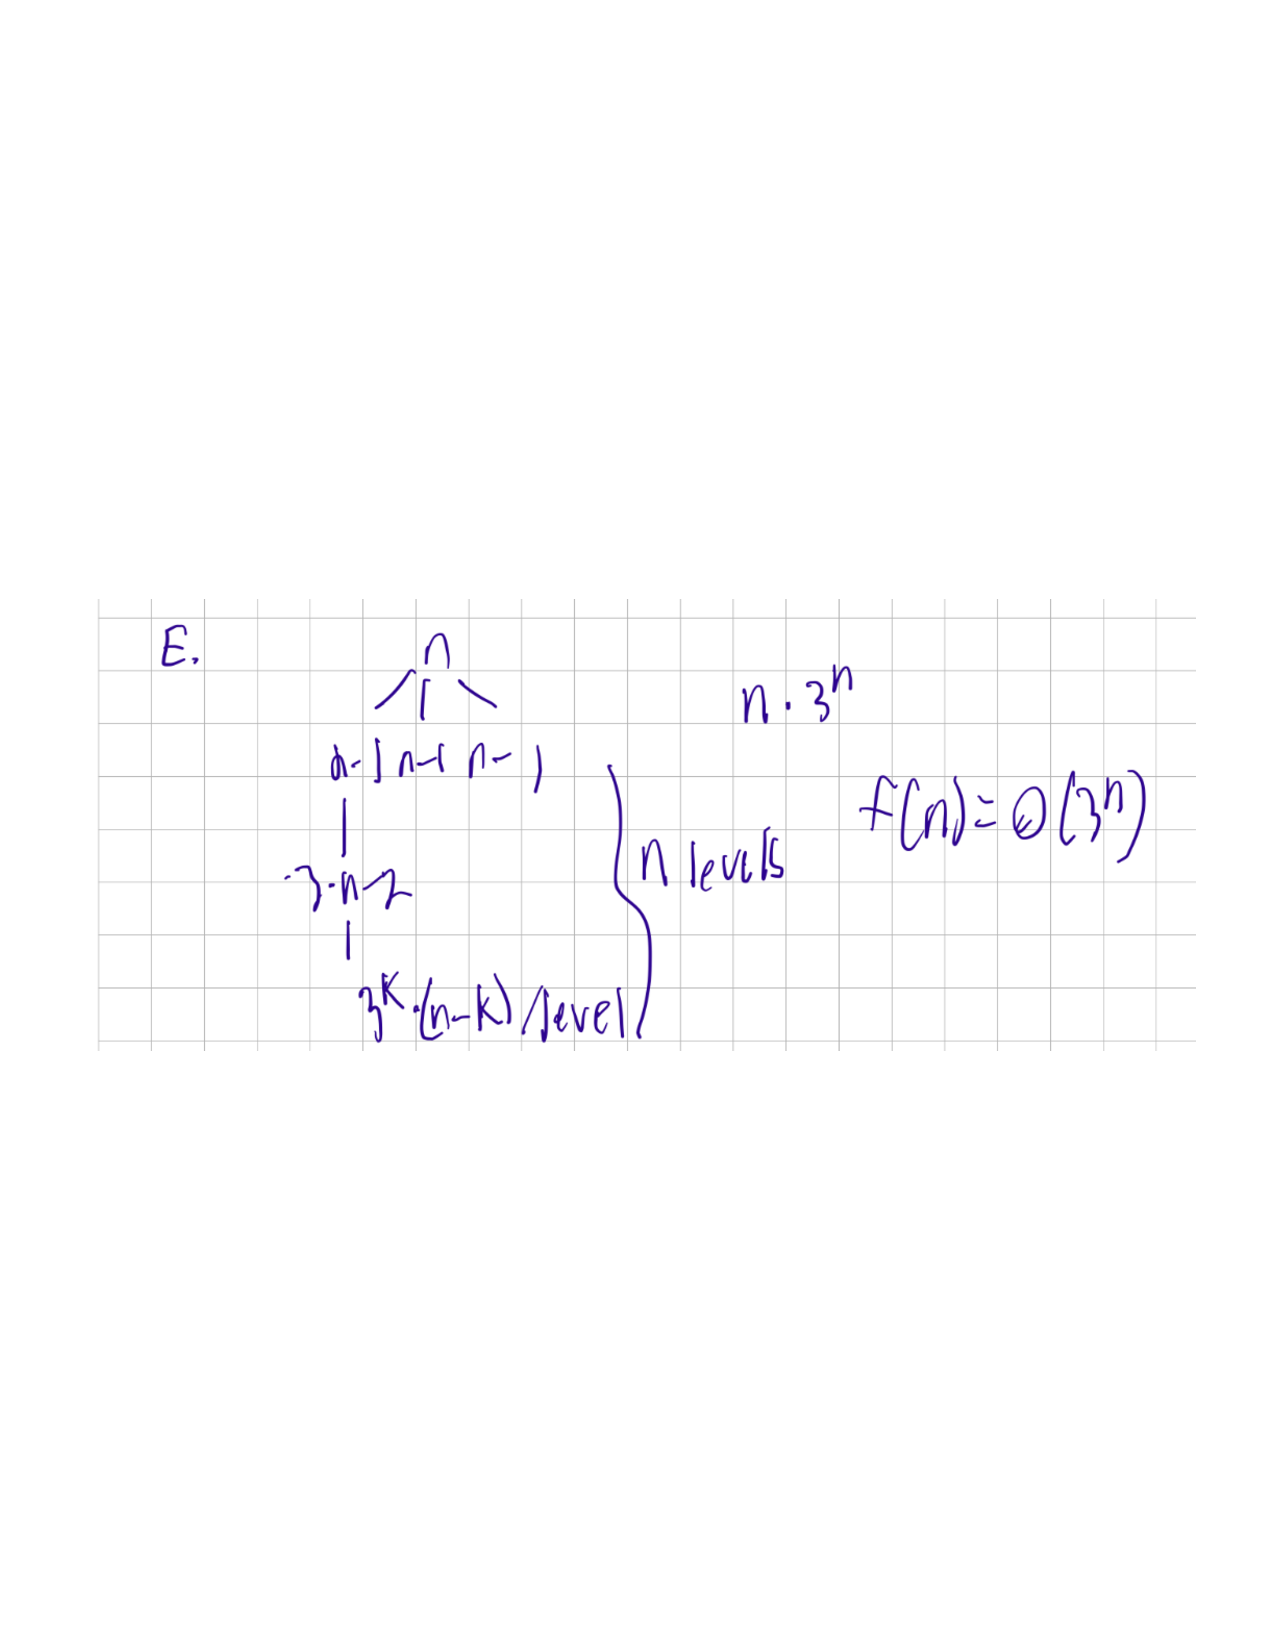
\includegraphics[width=0.5\textwidth]{problemE.pdf}}{No Figure Yet}
              \caption{Recursion tree for algorithm $E$.}
            \end{figure}

          \end{solution}

      \end{enumerate}

      For each algorithm, write a recurrence for its runtime and \emph{use the recursion tree method} to solve this recurrence and find the \emph{tightest asymptotic} upper bound on runtime of the algorithm. \grade{25}
    \end{problem}

    \smallskip

    \begin{problem}
      Each of the algorithms below takes as input a positive integer $n$ and then performs some steps. For each algorithm, state the running time of the algorithm as a function of $n$, using $\Theta$-notation.\\ \grade{15}

    \begin{enumerate}[label =\alph*)]
      \item
        \begin{itemize}
          \item For $i = 1$ to $n/3$
            \begin{itemize}
              \item $j \gets 10$
              \item While ($j \leq i/20$)
                \begin{itemize}
                  \item Do placeholder stuff that takes $O(1)$ time
                  \item $j \gets j + 10$
                \end{itemize}
            \end{itemize}
        \end{itemize}

        \begin{solution}
          This is just $O(n^2)$ because the outer loop runs (some multiple of) n times and so does the inner loop, which approaches n*n or $O(n^2)$
        \end{solution}

      \item

        \begin{itemize}
          \item While ($n \geq 1$)
            \begin{itemize}
              \item $n \gets n/3$
              \item do placeholder stuff that takes $O(1)$ time.
            \end{itemize}
        \end{itemize}
        \begin{solution}
          \

          $f(n) = \theta(log_3 n)$ This is true because this is just repeatedly dividing by 3 until n is a small number. repeated division in a loop gives log time.
        \end{solution}

      \item
        \begin{itemize}
          \item While ($n \geq 2$)
            \begin{itemize}
              \item $n \gets \sqrt{n}$
              \item Do placeholder stuff that takes $O(1)$ time.
            \end{itemize}
        \end{itemize}

        \begin{solution}
          \

          $f(n) = \theta(\log\log n)$ This is true because we are terminating the loop when our index variable reaches a small value and our index value is decremented by repeatedly taking the square root, which corresponds to $log(log n)$ reps
        \end{solution}

      \item

        \begin{itemize}
          \item For $i = 1$ to $n$
            \begin{itemize}
              \item For $j = 1$ to $i^2$
                \begin{itemize}
                  \item Do placeholder stuff that takes $O(1)$ time
                \end{itemize}
            \end{itemize}
        \end{itemize}
        \begin{solution}
          \

          $f(n) = \theta(n^3)$

          This is because the outer loop runs n times and the inner runs somewhere in the order of $n^2$ times.
        \end{solution}

      \item
        \begin{itemize}
          \item For $i = 1$ to $n$
            \begin{itemize}
              \item For $j = 1$ to $\log(i)$
                \begin{itemize}
                  \item For $k = 1$ to $n$
                    \begin{itemize}
                      \item Do placeholder stuff that takes $O(1)$ time
                    \end{itemize}
                \end{itemize}
            \end{itemize}
        \end{itemize}
        \begin{solution}
          $f(n) = \theta(n^2 * \log n)$ This is because the inner and outermost loops run n times and the middle on runs log n times and $n*n*\log n = n^2 \log n$
        \end{solution}

    \end{enumerate}

  \end{problem}

  \begin{problem}
    In this problem, we consider a non-standard sorting algorithm called the \emph{Slow Sort}. Given an array $A[1:n]$ of $n$ integers, the algorithm is as follows:

    $\bullet$ \textbf{Slow-Sort}$(A[1:n])$:
    \begin{enumerate}
      \item If $n < 100$, run merge sort (or selection sort or insertion sort) on $A$.
      \item Otherwise, run \textbf{Slow-Sort}$(A[1:n-1])$, \textbf{Slow-Sort}$(A[2:n])$, and \textbf{Slow-Sort}$(A[1:n-1])$ again.
    \end{enumerate}

    We now analyze this algorithm.

    \begin{enumerate}
      \item [(a)] Prove the correctness of  \textbf{Slow-Sort}. \grade{15}

        \begin{solution}
          \

          For the trivial cases where $n<100$, slow sort is proven because it just runs merge sort, which is proven.

          We then have the other basic case where $n = 101$

          In this case, we first sort an array of size 100 with all but the last item of the array in it.

          The result of this is an array that is sorted except for the position of the last element. The first element in the array is (most likely) the smallest in the array *unless* the unsorted item is.

          Now we sort an array of size 100 with all but the first item of the array in it. This sorting run will do almost nothing except for insert the last item in the array where it belongs. The array is most likely now sorted, unless the final item (of the full 101 item array) happens to have been the smallest, in which case it is at the front of the subarray.

          Now we sort an array of size 100 with all but the last item of the array in it. This will do nothing except for move the correct item into the front of the array as the smallest item. The 101 item array is now solved.

          It now follows by induction that all arrays larger than this will devolve into this fundamental case.
        \end{solution}

      \item [(b)] Write a recurrence for  \textbf{Slow-Sort} and use the recursion tree method to solve this recurrence and find the \emph{tightest asymptotic} upper bound on the runtime of \textbf{Slow-Sort}. \grade{10}

        \begin{solution}
          $T(n) = 3T(n-1)$

          $f(n) = O(3^n)$

          \begin{figure}[H]
            \centering
            \IfFileExists{problem4.pdf}{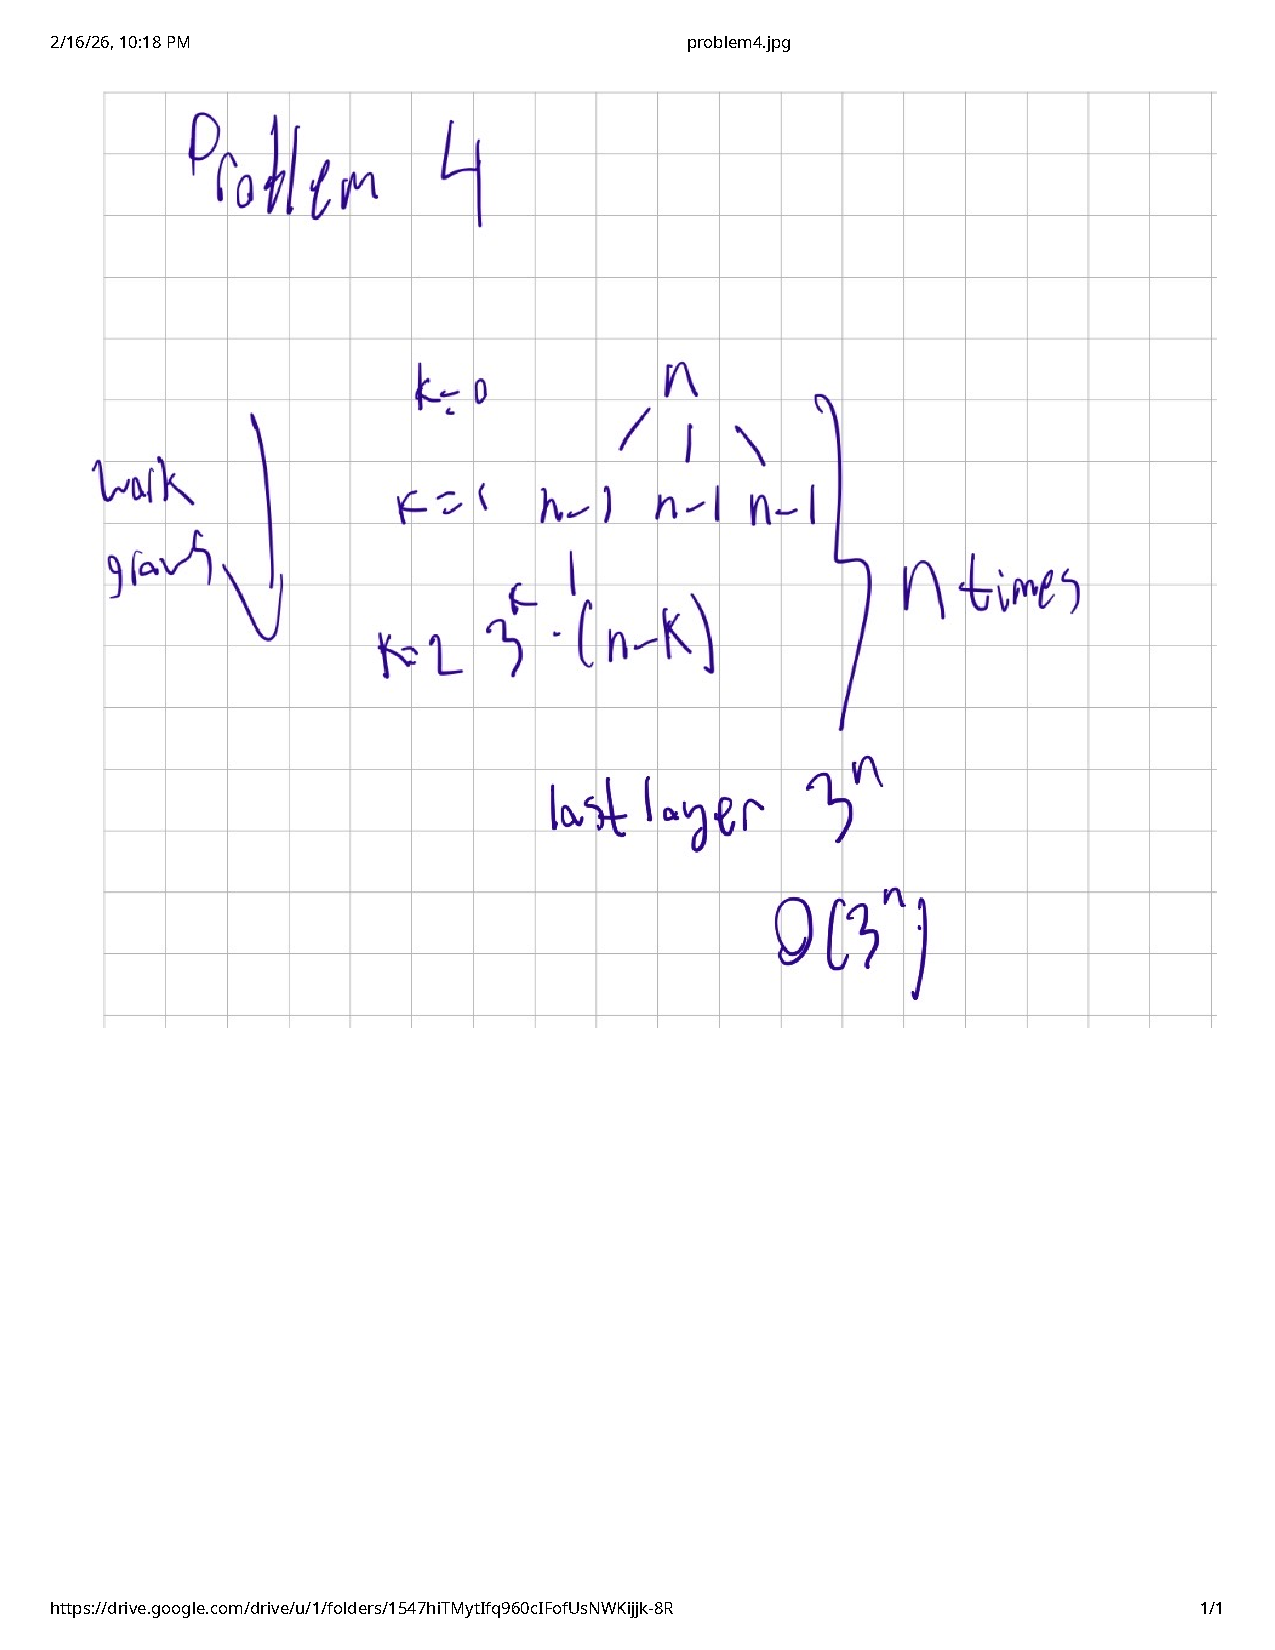
\includegraphics[width=0.5\textwidth]{problem4.pdf}}{No Figure Yet}
            \caption{Recursion tree for algorithm $A$.}
          \end{figure}
        \end{solution}

    \end{enumerate}
  \end{problem}

  \smallskip

  \begin{problem}
    Karatsuba multiplication reduces the time complexity of multiplying two $n$-digit numbers to $O(n^{\log_2 3}) \approx O(n^{1.585})$, using the recurrence:
    \[
      T(n) = 3T(n/2) + O(n)
    \]
    The algorithm splits the numbers as follows:
    \[
      x = x_1 \cdot 10^{n/2} + x_0, \quad y = y_1 \cdot 10^{n/2} + y_0
    \]
    and computes three products: $x_0 \cdot y_0$, $x_1 \cdot y_1$, and $(x_0 + x_1) \cdot (y_0 + y_1)$.

    Two values you are multiplying might be n/2 + 1 digits each, rather than n/2 digits, since the addition might have led to a carry. For instance compute $(x_1 + x_0)(y_1 + y_0)$ for $x = 53$ and $y = 52$. Notice the carry and the extra digit. So the recurrence will be \[
      T(n) = 2T(n/2) + T(n/2+1) + O(n)
    \]

    Prove that this issue won't affect our analysis and we still $O(n^{\log_2 3})$ complexity. \grade{20}

    \begin{solution}
      This is true because the $n/2 +1 \approx n/2$ and therefore as $n \to \infty$ that difference is irrelevant.

      Or, more formally:

      $3T(n/2) + O(n) = 2T(n/2) + T(n/t+1)$

      $T(n/2) = T(n/2+1)$

      $\lim_{n \to \infty} \frac{\frac{n}{2}}{\frac{n}{2} + 1} = 1$

    \end{solution}

  \end{problem}

  \begin{problem}
    Toom-Cook multiplication generalizes Karatsuba by dividing numbers into more parts. The Toom-3 algorithm splits two $n$-digit numbers $x$ and $y$ into three smaller parts:
    \[
      x = x_2 \cdot 10^{2k} + x_1 \cdot 10^k + x_0, \quad y = y_2 \cdot 10^{2k} + y_1 \cdot 10^k + y_0
    \]

    If we multiply we need to perform $9$  multiplications $x_iy_j$ of size $n/3$.

    \begin{enumerate}
      \item Write down the recurrence relation for the time complexity of the simple divide and conquer algorithm and solve it.

      \item Toom-3 algorithm instead only uses $5$ smaller multiplications to calculate all the $9$ products needed. Find the time complexity of Toom-3.

    \end{enumerate}

  \end{problem}\grade{20}
  \begin{solution}
    \

    1.

    $T(n) = 9T(\frac{n}{3}) + O(N)$

    $T(n) = O(n^{\log_3 9})$

    $T(n) = O(n^{2})$

    \hrule
    2.

    $T(n) = 5T(\frac{n}{3}) + O(N)$

    $T(n) = O(n^{\log_3 5})$

    $T(n) \approx O(n^{1.46})$
  \end{solution}

  \finishline

  \begin{challenge}
    We have an $n$-story building and a series of magical vases that work as follows: there is some unknown level $L$ in the building that if we throw these vases down from any of the levels $L,L+1,\ldots,n$, they will definitely break; however,
    no matter how many times we throw the vases down from any level below $L$ nothing will happen them. Our goal in this question is to determine this level $L$ by throwing the vases from different levels of the building (!).

    For each of the scenarios below, design an algorithm that uses asymptotically the smallest number of times we throw a vase (so the measure of efficiency for us is the number of vase throws).
    \begin{enumerate}
      \item[(a)] When we have only one vase. Once we break the vase, there is nothing else we can do. \grade{+2}

        From floor 1 to n, throw the vase. When it breaks, we have found L.
        This is $O(n)$. It must be so given that we may only use one vase.

      \item[(b)] When we have  four vases. Once we break all four vases, there is nothing else we can do. \grade{+4}

        Throw from n/2. If it breaks, throw from n/4. If it doesn't, throw from 3n/4.

        From this point, throw again. If it breaks, throw from the halfway point above where we just threw from. Otherwise, throw from the lower one.

        Repeat this one more time, from the new halfway point. If it breaks, throw from the bottom of the half below the level we were just on and go to each floor ascending. If it doesn't throw from each floor above in ascending order. We find L. This is $O(n/8)$ which is still basically $O(n)$
      \item[(c)] When we have an unlimited number of vases.  \grade{+4}
        Just use binary search. Throw from the middle. If it breaks throw from the middle of the lower half. If not throw from the middle of the upper half.

        This is O(logn).
    \end{enumerate}
  \end{challenge}

  \end{document}